\begin{frame}
    \frametitle{Method of Fragments}
    \only<1-2>{
        \centering
        \only<1>{\def\fraglevel{0}}
        \only<2>{\def\fraglevel{1}}
        \includestandalone{fig/montague-fragments}

        \begin{minipage}[t][2cm]{\textwidth}\vspace{1em}
            How do we get from messy language to formal logic?\\[0.5em]
            \emph{Montague}~\cite{Montague:efl70}: Look at a ``nice'' subset
            and map into logic.
        \end{minipage}
    }

    \only<3>{
        \centering
        \def\fraglevel{1}
        \includestandalone{fig/montague-fragments}
        
        \begin{minipage}[t][2cm]{0.6\textwidth}\vspace{1em}
            \str{Ahmed paints and Berta is quiet.}\\[0.5em]
            \str{Ahmed doesn't paint.}
        \end{minipage}\hfill
        \begin{minipage}[t][2cm]{0.39\textwidth}\vspace{1em}
            $p(a) \wedge q(b)$\\[0.5em]
            $\neg p(a)$
        \end{minipage}
    }

    \only<4>{
        \centering
        \def\fraglevel{2}
        \includestandalone{fig/montague-fragments}
        
        \begin{minipage}[t][2cm]{0.6\textwidth}\vspace{1em}
            \str{Every student paints and is quiet.}\\[0.5em]
            \str{Nobody paints.}
        \end{minipage}\hfill
        \begin{minipage}[t][2cm]{0.39\textwidth}\vspace{1em}
            $\forall x.s(x) \Rightarrow (p(x) \wedge q(x))$\\[0.5em]
            $\neg \exists x.p(x)$
        \end{minipage}
    }

    \only<5>{
        \centering
        \def\fraglevel{3}
        \includestandalone{fig/montague-fragments}

        \begin{minipage}[t][2cm]{0.6\textwidth}\vspace{1em}
            \str{Ahmed isn't allowed to paint.}\\[0.5em]
            \str{Ahmed and Berta must paint.}
        \end{minipage}\hfill
        \begin{minipage}[t][2cm]{0.39\textwidth}\vspace{1em}
            $\neg\lozenge p(a)$\\[0.5em]
            $(\square p(a)) \wedge \square p(b)$
        \end{minipage}
    }
\end{frame}


\begin{frame}
    \frametitle{Method of Fragments}
    {\color{hlfont}Hand-waving} is problematic:

    \hspace{2em}\str{Ahmed paints. He is quiet.}
    {$\quad\stackrel{?}{\leadsto}\quad$ \color{logicfont} $p(a)\wedge q(a)$}

    \vspace{1.2em}
    {\color{hlfont}Montague}: Specify
    \begin{itemize}
        \item grammar,\com{fixes NL subset}
        \item target logic,
        \item semantics construction.\com{maps parse trees to logic}
    \end{itemize}

    {
        \centering
        \vspace{0.3em}
        {\itshape\footnotesize Example from~\cite{Montague:tptoqi73}}

        \vspace{0.2em}\fbox{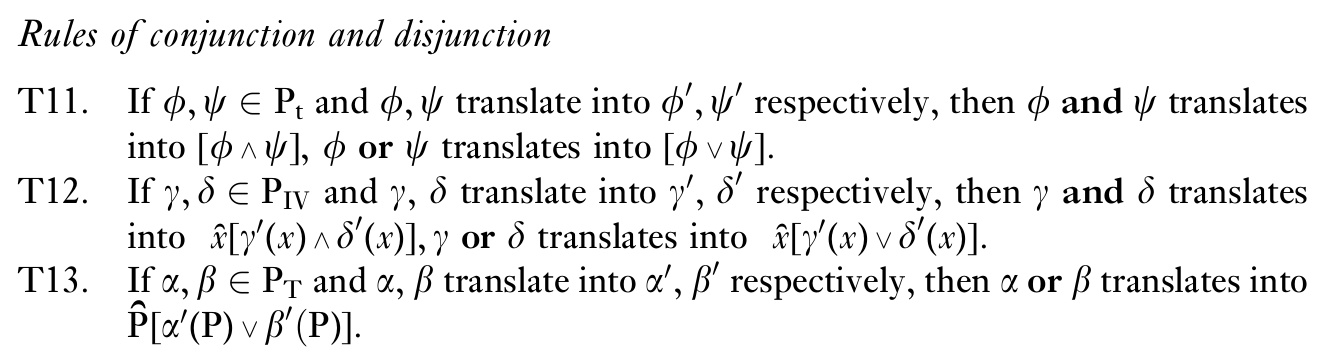
\includegraphics[trim=0 0 0 80,clip,width=0.7\textwidth]{fig/montague-tptoqioe.png}}

        \vspace{1.2em}
        Claim: That doesn't scale well $\leadsto$ \textbf{We need {\color{hlfont}prototyping}!}
    }

    % \newcommand\VP{\text{\upshape\tiny VP}}
    % \hspace{2em}$\llbracket\text{\strplain{$P_{\VP}$ and $Q_{\VP}$}}\rrbracket_{\VP} = \lambda x. \llbracket\text{\strplain{$P_{\VP}$}}\rrbracket(x) \wedge \llbracket\text{\strplain{$Q_{\VP}$}}\rrbracket(x)$
\end{frame}


\begin{frame}[fragile]
    \frametitle{NLU Prototyping}
%     \begin{lstlisting}[mathescape,keywords=translate,keywordstyle=\bf,
%                        morestring={[d]"}, stringstyle=\it,showstringspaces=false]
    \begin{center}
\fbox{\parbox{0.7\textwidth}{{\ttfamily
> \textbf{translate} {\color{nlfont}"Every student paints and is quiet."}\\
\color{logicfont}$\forall x.s(x)\Rightarrow(p(x)\wedge q(x))$
}}}
    \end{center}

%     \end{lstlisting}
    \vspace{1.5em}
    \begin{itemize}
        \item Traditionally done in Prolog/Haskell
        \begin{itemize}
            \item[$\raa$] requires a lot of work
        \end{itemize}
            \item A dedicated framework might be better
        \begin{itemize}
            \item[$\raa$] only partial solutions exist
        \end{itemize}
        \item Can we combine existing partial solutions? % \com{Research Question}
        \begin{itemize}
            \item[$\leadsto$] GLIF
        \end{itemize}
    \end{itemize}
\end{frame}

